\subsection{Results for Trajectories Estimated Using Speed, Heading, and Time}
%\label{subsec:speed_actual_dir_results}
%\vspace{10pt}

Figure~\ref{fig:traj_speed_actual_dir_RMSE} represents the $p$-values for the Wilcoxon signed-rank test on RMSE values across $k$-fold validation datasets for the trajectories estimated using speed, heading, and time in the $k$-fold testing datasets using different RNN models, and forecasting times. Darker colors in grayscale represent a higher $p$-value in a range from $0$ to $1$. The values on the secondary diagonal are all equal to $1$ and black because models equal themselves.

\begin{figure}[!ht]
	\centering
	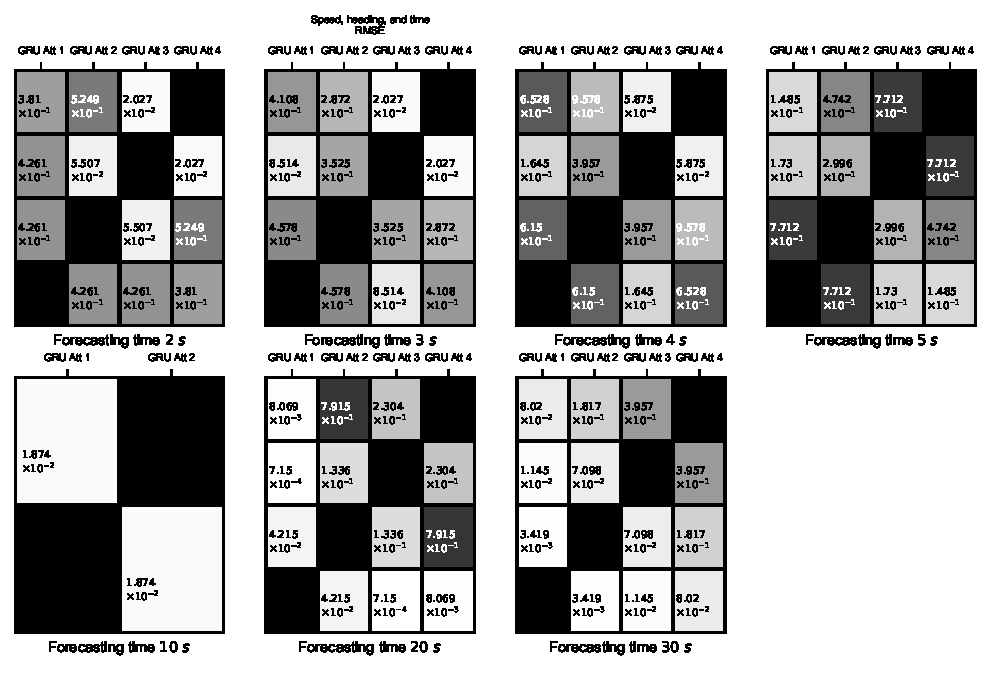
\includegraphics[width = 0.99 \linewidth]{traj_speed_actual_dir_RMSE.pdf}
	\caption{The $p$-values for the Wilcoxon signed-rank test on RMSE values across $k$-fold validation datasets for the trajectories estimated using speed, heading, and time in the $k$-fold testing datasets using different RNN models, and forecasting times. Darker colors in grayscale represent a higher $p$-value in a range from $0$ to $1$. The values on the secondary diagonal are all equal to $1$ and black because models equal themselves.}
	\label{fig:traj_speed_actual_dir_RMSE}
\end{figure}

The average RMSE in $\degree$ ($\times 10^{-2}$), with standard deviation in brackets, across $k$-fold validation datasets for the trajectories in the $k$-fold testing datasets estimated using speed, heading, and time, different RNN models, and forecasting times is listed in Table~\ref{tab:best_speed_actual_dir_RMSE}.

\begin{table}[!ht]
	\centering
	\resizebox{\linewidth}{!}{
		\begin{tabular}{|c|c|c|c|c|c|c|c|}
			\hline
			Model & $2$ $s$ & $3$ $s$ & $4$ $s$ & $5$ $s$ & $10$ $s$ & $20$ $s$ & $30$ $s$ \\ \hline
			\multirow{2}{*}{GRU Att 1} & $1.501$ & $1.524$ & $1.587$ & $\mathbf{1.598}$ & $\mathbf{1.745}$ & $\mathbf{2.657}$ & $7.659$ \\
			 & ($0.163$) & ($0.154$) & ($0.163$) & \textbf{(}$\mathbf{0.135}$\textbf{)} & \textbf{(}$\mathbf{0.108}$\textbf{)} & \textbf{(}$\mathbf{0.17}$\textbf{)} & ($6.196$) \\ \hline
			\multirow{2}{*}{GRU Att 2} & $1.495$ & $1.536$ & $1.586$ & $1.616$ & $1.818$ & $2.72$ & $\mathbf{3.919}$ \\
			 & ($0.161$) & ($0.177$) & ($0.173$) & ($0.165$) & ($0.192$) & ($0.19$) & \textbf{(}$\mathbf{0.589}$\textbf{)} \\ \hline
			\multirow{2}{*}{GRU Att 4} & $\mathbf{1.494}$ & $\mathbf{1.514}$ & $\mathbf{1.581}$ & $1.616$ & $1.842$ & $2.737$ & $5.269$ \\
			 & \textbf{(}$\mathbf{0.152}$\textbf{)} & \textbf{(}$\mathbf{0.163}$\textbf{)} & \textbf{(}$\mathbf{0.173}$\textbf{)} & ($0.15$) & ($0.125$) & ($0.238$) & ($4.403$) \\ \hline
		\end{tabular}
	}
	\caption{The average RMSE in $\degree$ ($\times 10^{-2}$), with standard deviation in brackets, across $k$-fold validation datasets for the trajectories in the $k$-fold testing datasets estimated using speed, heading, and time, different RNN models, and forecasting times.}
	\label{tab:best_speed_actual_dir_RMSE}
\end{table}

The GRU Att 1 model achieved the lowest RMSE for trajectories estimated using speed, heading, and time, and a forecasting time of $10$, $20$, and $5$ $s$ with average values and standard deviation (in brackets) that equal $17.45 \times 10^{-3}$ $\degree$ ($1.08 \times 10^{-3}$ $\degree$), $26.57 \times 10^{-3}$ $\degree$ ($1.7 \times 10^{-3}$ $\degree$), and $15.98 \times 10^{-3}$ $\degree$ ($1.35 \times 10^{-3}$ $\degree$) respectively.

The GRU Att 1 model does not have a statistically significantly different RMSE than the GRU Att 2 model for speed, heading, and time using a forecasting time of $10$ $s$, with a $p$-value equaling $1.874 \times 10^{-2}$.

\markertable{tab:\label{tab:RMSE:speed:actual:dir:p:10}}

The GRU Att 1 model does not have a statistically significantly different RMSE than the GRU Att 2, GRU Att 3, and GRU Att 4 models for speed, heading, and time using a forecasting time of $20$ $s$, with $p$-values equaling $4.215 \times 10^{-2}$, $7.15 \times 10^{-4}$, and $8.069 \times 10^{-3}$.

\markertable{tab:\label{tab:RMSE:speed:actual:dir:p:20}}

The GRU Att 1 model does not have a statistically significantly different RMSE than the GRU Att 2, GRU Att 3, and GRU Att 4 models for speed, heading, and time using a forecasting time of $5$ $s$, with $p$-values equaling $7.712 \times 10^{-1}$, $1.73 \times 10^{-1}$, and $1.485 \times 10^{-1}$.

\markertable{tab:\label{tab:RMSE:speed:actual:dir:p:5}}

The GRU Att 2 model achieved the lowest RMSE for trajectories estimated using speed, heading, and time, and a forecasting time of $30$ $s$ with an average value and standard deviation (in brackets) that equals $39.19 \times 10^{-3}$ $\degree$ ($5.89 \times 10^{-3}$ $\degree$).

The GRU Att 2 model does not have a statistically significantly different RMSE than the GRU Att 1, GRU Att 3, and GRU Att 4 models for speed, heading, and time using a forecasting time of $30$ $s$, with $p$-values equaling $3.419 \times 10^{-3}$, $7.098 \times 10^{-2}$, and $1.817 \times 10^{-1}$.

\markertable{tab:\label{tab:RMSE:speed:actual:dir:p:30}}

The GRU Att 4 model achieved the lowest RMSE for trajectories estimated using speed, heading, and time, and a forecasting time of $2$, $3$, and $4$ $s$ with average values and standard deviation (in brackets) that equal $14.94 \times 10^{-3}$ $\degree$ ($1.52 \times 10^{-3}$ $\degree$), $15.14 \times 10^{-3}$ $\degree$ ($1.63 \times 10^{-3}$ $\degree$), and $15.81 \times 10^{-3}$ $\degree$ ($1.73 \times 10^{-3}$ $\degree$) respectively.

The GRU Att 4 model does not have a statistically significantly different RMSE than the GRU Att 1, GRU Att 2, and GRU Att 3 models for speed, heading, and time using a forecasting time of $2$ $s$, with $p$-values equaling $3.81 \times 10^{-1}$, $5.249 \times 10^{-1}$, and $2.027 \times 10^{-2}$.

\markertable{tab:\label{tab:RMSE:speed:actual:dir:p:2}}

The GRU Att 4 model does not have a statistically significantly different RMSE than the GRU Att 1, GRU Att 2, and GRU Att 3 models for speed, heading, and time using a forecasting time of $3$ $s$, with $p$-values equaling $4.108 \times 10^{-1}$, $2.872 \times 10^{-1}$, and $2.027 \times 10^{-2}$.

\markertable{tab:\label{tab:RMSE:speed:actual:dir:p:3}}

The GRU Att 4 model does not have a statistically significantly different RMSE than the GRU Att 1, GRU Att 2, and GRU Att 3 models for speed, heading, and time using a forecasting time of $4$ $s$, with $p$-values equaling $6.528 \times 10^{-1}$, $9.578 \times 10^{-1}$, and $5.875 \times 10^{-2}$.

\markertable{tab:\label{tab:RMSE:speed:actual:dir:p:4}}

